\section{Related Work}

Photo retouching has been explored in image processing and computer vision communities under different domains, such as photo enhancement and image-to-image translation. Below, we first discuss recent methods on photo enhancement and then image-to-image map definitions with the main focus on learning-based methods.

\subsection{Digital Photo Enhancement}
% \myworries{Check Rafals' paper -- is it global tone mapping, where to put it in the related work}
\paragraph{Global image enhancement.} Colour and tone transfer has been considered a very effective technique to improve the perceptual quality of photos with pre-defined rules or examples \cite{Faridul14ASurvey, mustafa2022distilling}. 

Earlier methods typically apply global changes and adjust image statistics \cite{Bychkovsky11Learning, Bae06Two, Pitie05NDimensional,Pitie07Automated,Reinhard01Color,Sunkavalli10Multi, he2020conditional, park2018distort}, e.g., mean and standard deviation, without considering image content and local variations \cite{CohenOr06Color}. These methods, in general, transfer colour changes, ignoring edits in fine details. On the other hand, the proposed method learns a mapping per frequency band, capturing transfers even in high frequencies. \citeauthor{Bychkovsky11Learning} \cite{Bychkovsky11Learning} collected the MIT-Adobe FiveK dataset of 5,000 photographs and their retouched versions by five artists. The authors propose a regression model to learn artists' retouching styles from before-retouched pairs. \citeauthor{chen2017fast} \cite{chen2017fast} introduce a fully-convolutional neural network model to learn global image processing operators, such as photographic style, nonlocal dehazing, and pencil drawing. \citeauthor{Hu18Exposure} \cite{Hu18Exposure} presents a photo retouching pipeline for various post-processing operations, where global adjustment curves are approximated. The authors propose a deep reinforcement learning approach to model users' edit preferences from a given photo collection. 
 
Nevertheless, global transfers cannot capture local and regional variations in a photo \cite{CohenOr06Color}.They may result in artifacts when the local target regions of the example and input images do not match. In this method, we adapt the mappings to each image patch separately, thus accurately capturing local edits in intricate details.

\paragraph{Local context-aware image enhancement.} 
 To capture local variations, different methods have been proposed, such as learning local representative color transform \cite{kim2021representative}, estimating an image-to-illumination mapping with a local feature extractor \cite{wang2019underexposed}, local histogram matching \cite{Shapira13Image}, segmentation \cite{Laffont14Transient,Tai07Soft}, combining and learning pre-defined filters \cite{Berthouzoz11AFramework,Chen18Deep,Huang14Parametric,Omiya18Learning,Saeedi18Multimodal} or with further user guidance \cite{An10User,Pouli11Progressive,Tai05Local}, detection or learning of image semantics and context \cite{Gharbi17Deep,Hwang12Context,Kaufman12Content,Nam17Deep,Yan14Automatic,Zhu18Automatic}, matching \cite{HaCohen11Nonrigid}, or precise alignment \cite{Kagarlitsky09Piecewise, Shih13Data}. 
 
 Furthermore, recent work has focused on learning global and local adjustments via spatially-varying filters \cite{moran2020deeplpf, Gharbi17Deep, chen2018deep, shaham2021spatially, li2020lapar}. \citeauthor{chen2018deep} \cite{chen2018deep} introduce a global feature extraction layer along with per-pixel adjustments to enhance photos. Bilateral guided joint upsampling \cite{chen2016bilateral} also allows for local and global image processing with an encoder-decoder approach. HDRNet \cite{Gharbi17Deep} learn content-aware, global, and local adjustments via a two-stream convolutional architecture, which extracts local and global features separately to fit local affine transformations and encode the high-level description of images, respectively. Also, \citeauthor{moran2020deeplpf} \cite{moran2020deeplpf} propose to learn the parameters of three different spatially local filters to automatically enhance photos. 

Local color and tone adjustments might still be insufficient to capture intricate details \cite{Bae06Two}. Transfer of such details typically requires a dense matching \cite{HaCohen11Nonrigid} or alignment between example and input images \cite{Shih14Style}. To achieve either dense matching or alignment, methods constrain their datasets to contain very similar example and input images, for example, faces with similar characteristics and views~\cite{Shih14Style}. On the other hand, this framework does not require dense correspondences between input and example images but still transfers intricate details. It accurately represents such complex mappings with an operator summing the effects of various transformations multiplied with corresponding patch-adaptive weights, applied at multiple frequency bands.

\paragraph{Differentiable image processing pipelines.}
To have more flexibility and control over the rendering process, methods based on image signal processors (ISP)s have been proposed to enhance photos. In both \cite{tseng2019hyperparameter, yu2021reconfigisp}, hyperparameters of an ISP are optimized. Different from \cite{tseng2019hyperparameter}, which only applies to a fixed pipeline, \citeauthor{yu2021reconfigisp} \cite{yu2021reconfigisp} can explore different ISP architectures. Furthermore, \citeauthor{tseng2022neural} \cite{tseng2022neural} model a commercial raw processing pipeline with a series of neural networks to render sRGB images from raw inputs. As we assume example and input images to be processed RGB images rather than raw data, I refrain from comparing our method with such ISP-based methods.


\subsection{Defining Maps between Images}

\paragraph{Unsupervised methods.} Some learning-based techniques only require one or more examples of retouched photos without their before examples to learn the transfer. Such unsupervised methods capture a certain style by decomposing images into a reflection map and an illumination map~\cite{ma2021retinexgan},
extracting and recomposing band representations of training images~\cite{yang2020fidelity}, regularizing unpaired training using information extracted from the input~\cite{9334429}, segmenting the image into semantic regions~\cite{Liu16Makeup}, adaptive image regions~\cite{Frigo16Split}, learning semantic and global features~\cite{Chen18Deep}, progressively translating image from coarse to fine via pyramids of generative models \cite{lin2020tuigan}, or utilizing artistic principles and pre-defined filters~\cite{Zhang13Style,Hu18Exposure}. These methods transfer pre-defined elements of the desired style, or global color and tone. Defining the desired style and the content of the input image that is to remain is challenging. Hence, these methods typically assume prior knowledge of the type of desired adjustments. Even then, capturing the retouching edits in details remains out of scope since these methods are mainly designed for domain transfer, working on high level features of images. % TuiGAN: compare with our work, discuss how bady they perform in details although they work as single-shot --

As a weakly supervised method, \citeauthor{visual_attribute} \cite{visual_attribute} propose a technique based on image analogy \cite{Hertzmann01Image} to transfer the visual attributes, such as color, tone, texture, and style, across images that look very different but share similar semantic structures. Similar to this work, they also work with one example pair (A and B') to transfer the attributes. However, they rather focus on high-level features, disregarding the edits in intricate details.

\paragraph{Supervised methods.} 
For a conceivable representation, many supervised transfer methods require a large dataset of well-aligned example image pairs whose contents are very similar \cite{kim2021representative, wang2019underexposed}. However, finding or generating such a dataset is difficult as the content of images can change dramatically. Even with such a dataset, segmentation errors, unseen semantic regions, or image content can still change the results significantly \cite{10.1145/2790296}. In contrast, this framework allows users to choose the example pairs from which the desired style is learned, hence sidestepping the challenging semantics problem. Similar content and structures between example and input images lead to more natural transfers.


Convolutional neural networks (CNNs) are the de-facto model for image processing with supervised learning methods. While CNNs present state-of-the-art results in computer vision tasks, they are not required \cite{tolstikhin2021mlp}. MLP-based architectures have recently gained popularity in image classification and image-to-image translation. \citeauthor{cazenavette2021mixergan} \cite{cazenavette2021mixergan} propose the MLP-Mixer architecture that only uses simple MLP blocks to learn image classification. \citeauthor{cazenavette2021mixergan} \cite{cazenavette2021mixergan} also show an application of an MLP-based architecture for image synthesis. They adapt the MLP-Mixer architecture \cite{tolstikhin2021mlp} to perform unpaired image-to-image translation. The fact that MLP-based architectures attain competitive results in challenging vision tasks motivated me to explore the use of an MLP block as an alternative to CNNs in the context of photo retouching.

\section{Overview and Motivations}
\label{chap:motivations}

Given a pair of example images $X$ and $Y$, the aim is to learn a map $M$ such that $Y = M(X)$. The learned map can then be applied to a new input image $I$ to obtain the retouched output $O = M(I)$. 

The map is defined by 1) decomposing the example images into multiple feature maps $X_l$, $Y_l$ capturing details at different scales, such as coefficients at different bands of a Laplacian pyramid. 2) learning a separate mapping $M_l$ for each $X_l$, $Y_l$ pair in the patch space as a blending of transformation matrices with neural field based weights, all learned jointly. The overall map representation is illustrated in Figure~\ref{fig:modelT}.

For the transfer of edits, the $M_l$ are computed and applied to each patch of the decomposition $I_l$ of an input image $I$ to obtain the corresponding output patch of $O_l$. The patches are finally placed at their spatial locations and averaged to reconstruct each band $O_l$, which are summed to get the output image $O$.

The motivation behind designing such a map representation with frequency decomposition and transformation blending comes from studying the nature of retouching edits. 
\begin{itemize}
\item First, artists often decompose images into different frequency bands to have better control over structural and textural edits to details. For instance, they filter out the low frequency components to better enhance the details:

\begin{figure}[ht]
\centering
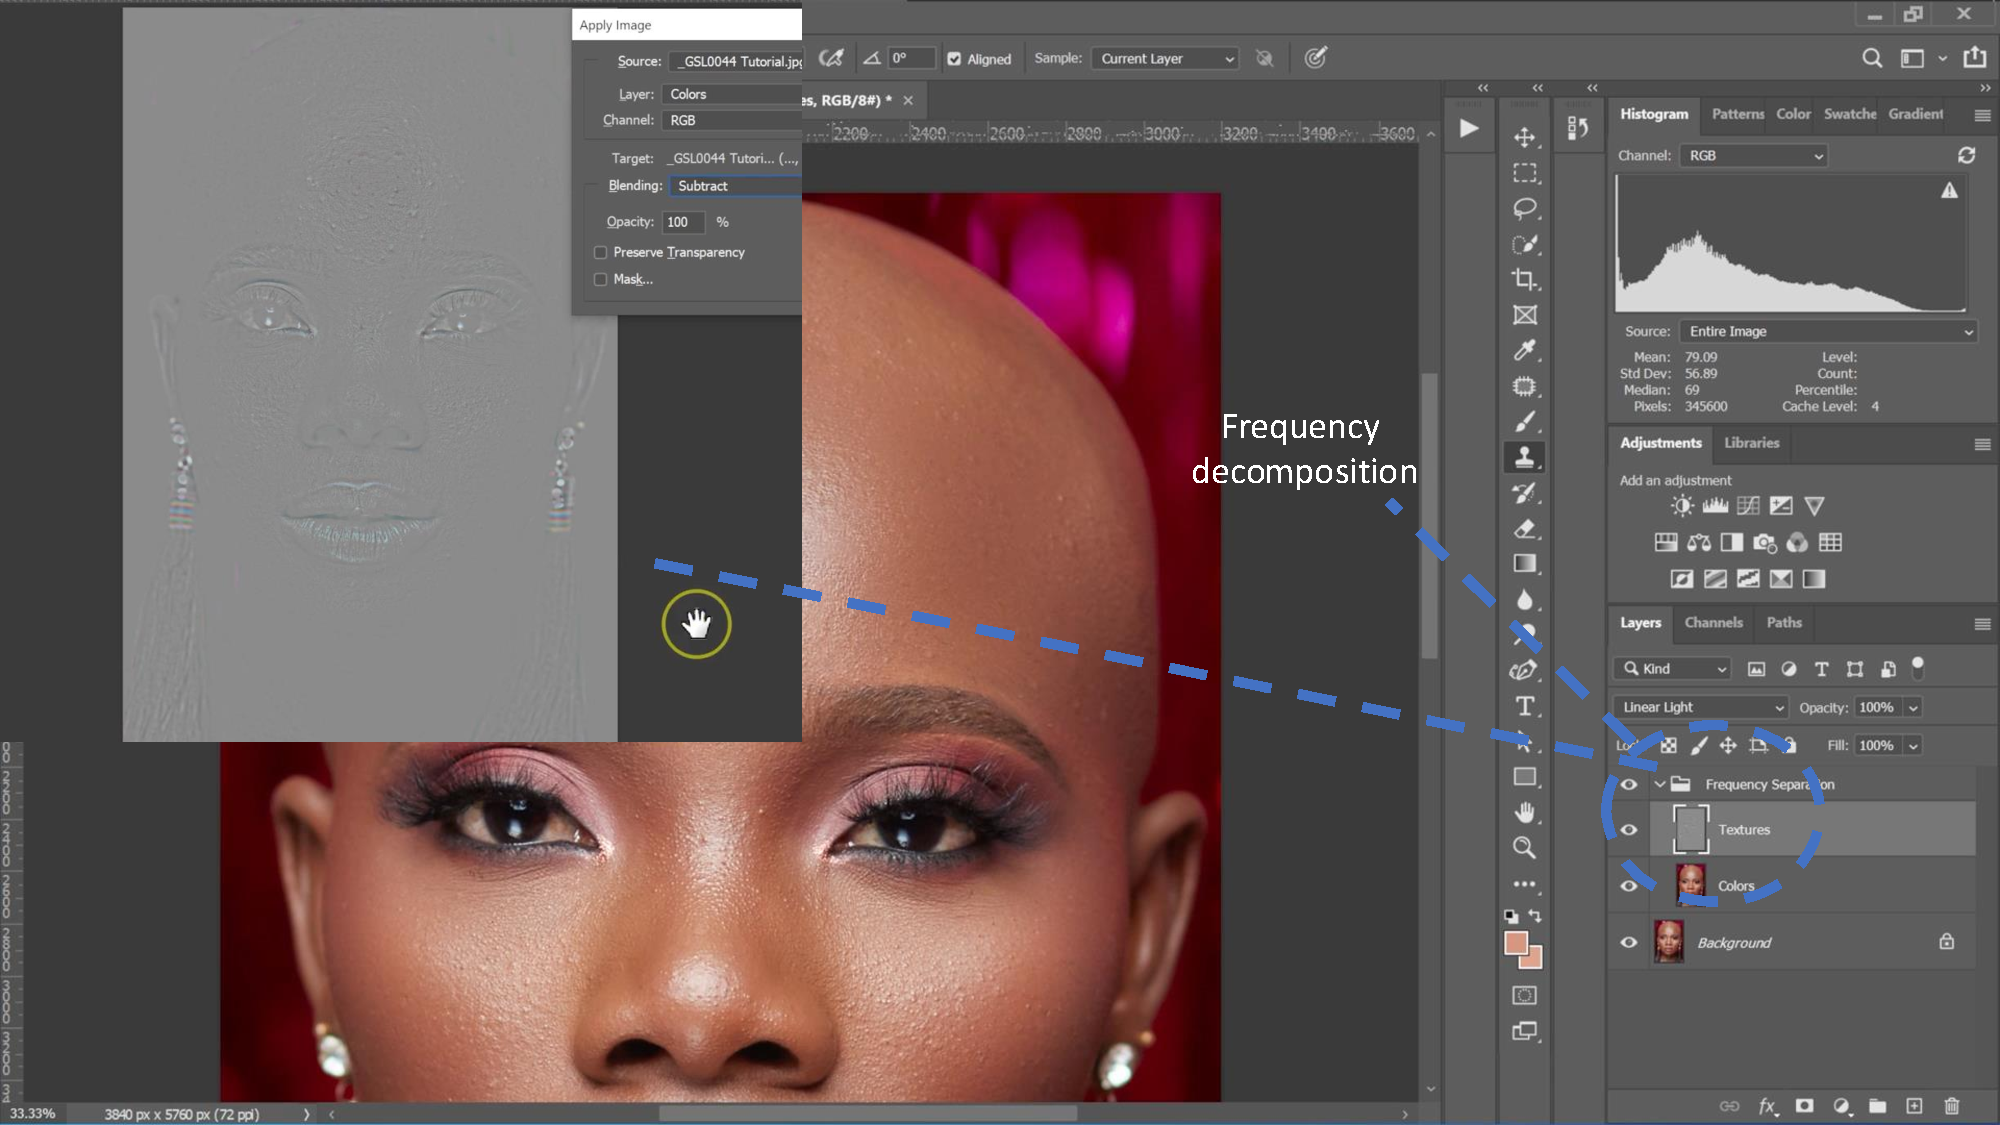
\includegraphics[width=\columnwidth]{Chapters/detail-retouching-figs/PS1.pdf}
    \caption{Frequency decomposition allows artists to have a higher control over different frequency components of an image. Here, the layer shown in the top-left corner is obtained by high-pass filtering of the portrait in the background. Screenshots from [Eustace Kanyanda, 2022].}

\label{fig:PS-high-pass}
\end{figure}

\item Second, image patches of similar content, e.g. skin or hair, are retouched similarly. This means similar patches in the patch space translate into similar edits. The proposed representation leads to a different transformation for patches of differing content. Local filters can offer such edits, where similar contents, such as pores, transform into a similar content, such as a smooth texture:
\begin{figure}[ht]
\centering
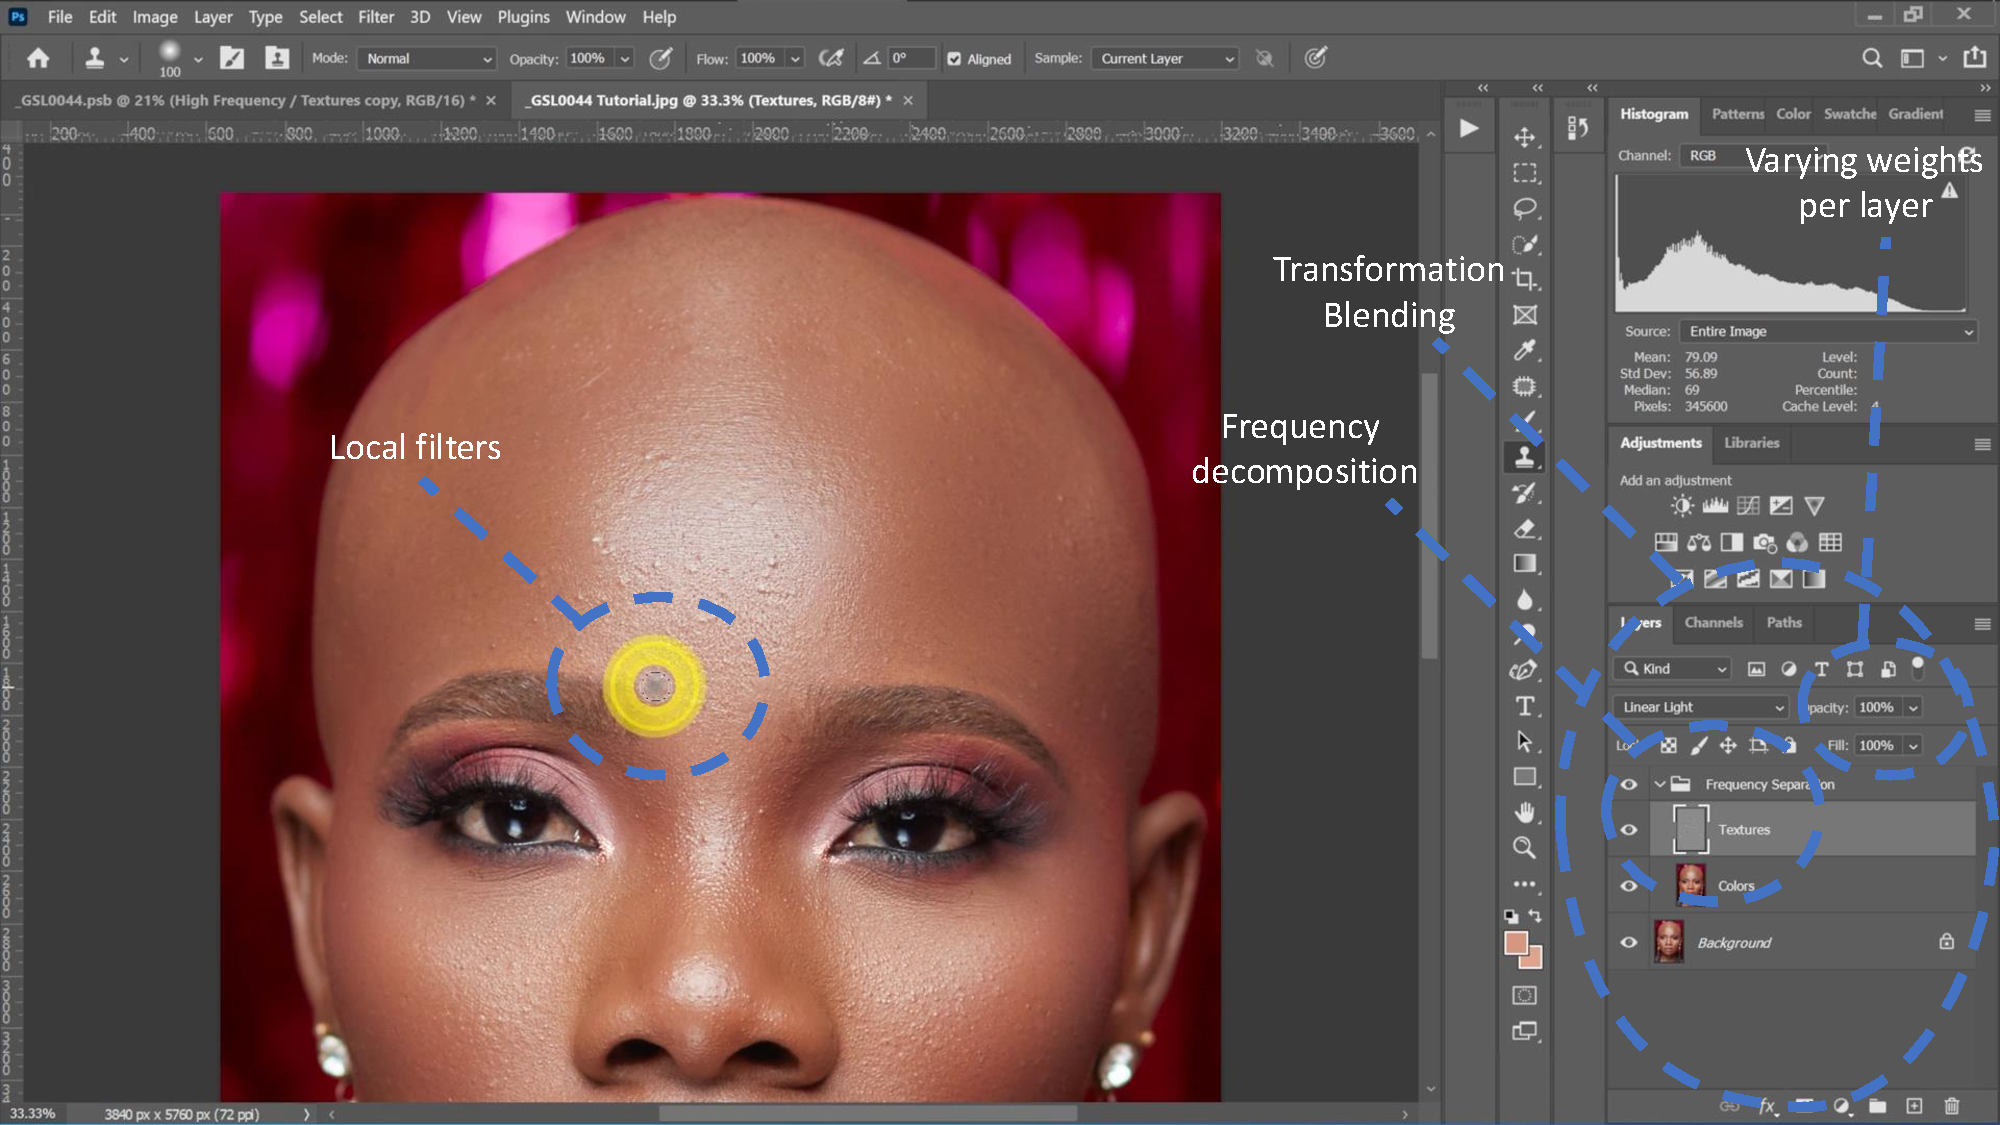
\includegraphics[width=\columnwidth]{Chapters/detail-retouching-figs/PS3.pdf}
    \caption{Local filters, such as brushes, help smoothing the skin by removing the undesired pores on the face. However, it is a tedious task for artists, requiring them to go through each of the visible pores.}

\label{fig:PS-brush}
\end{figure}

\item Third, these edits, global and local adjustments, are typically applied in separate layers and then blended with a subjective opacity value. The neural transformation blending with an MLP block outputting the weights per layer replicates the composition of different layers with their corresponding opacity values:

\begin{figure}[ht]
\centering
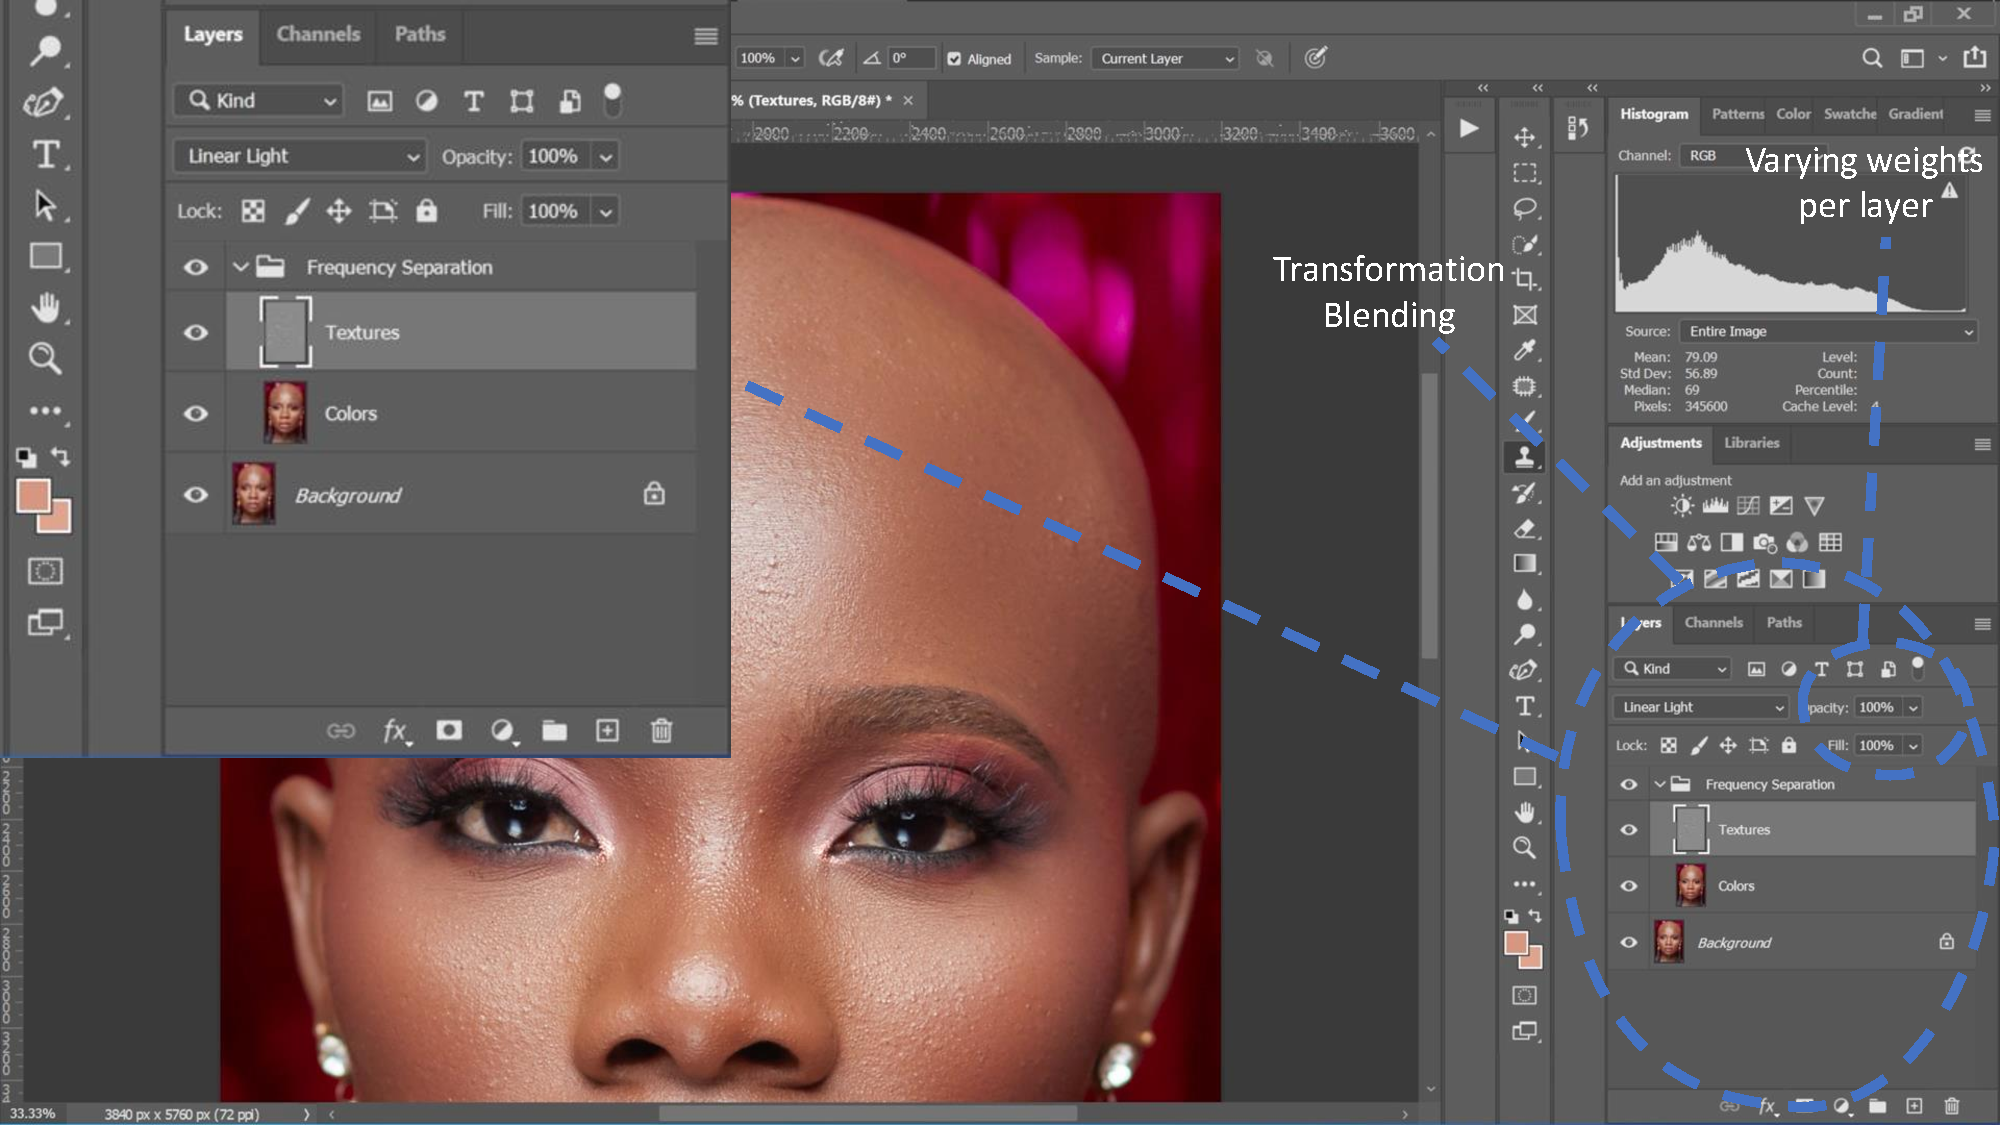
\includegraphics[width=\columnwidth]{Chapters/detail-retouching-figs/PS2.pdf}
    \caption{Artists usually work on separate layers, adjusting varying properties, such as texture, colour, etc. Later, these layers are blended together with their corresponding "opacity" values, shown in the box above the layers.}

\label{fig:PS-all-together}
\end{figure}

\end{itemize}
Although professional artist pipelines inspire this work, I illustrate in the next sections that this new image-to-image mapping representation can replicate the effect of and transfer edits for many filters.
